\section{Réseaux antagonistes génératifs}
\subsection{Généralités}
Un Réseau antagoniste génératif\cite{gan} (Generative Adversarial Networks (GAN)) est un réseau dont l'architecture s'inspire d'un problème issu de la \textit{Théorie des Jeux}, le \textit{Minimax}\footnote{Pour plus d'informations sur ce \textit{jeu}, consultez \url{http://people.maths.ox.ac.uk/griffit4/Math_Alive/3/game_theory3.pdf}}. Ses performances sont remarquables dans le cadre de la \textit{génération de données}, notamment les images. Ce réseau est composé de deux sous-réseaux: un \textit{Générateur} et un \textit{Discriminateur}.\\

\noindent L'objectif du \textit{Générateur} est de produire une donnée artificielle alors que le \textit{Discriminateur} doit dissocier les images réelles des images artificielles. Le réseau va ainsi apprendre en cherchant à améliorer ses deux sous-réseaux: un \textit{Descriminateur} plus efficace à détecter les \textit{faux} et un \textit{Générateur} plus efficace pour produire des \textit{faux} "invisibles". \\

\noindent Le \textit{Générateur} prend en entrée, un vecteur \textit{bruitée} $c(\theta) \in R^d$\footnote{Par convention, d est égal à 100} issu d'une distribution normale ou uniforme entre -1 et 1 avant de produire une donnée artificielle de même dimension que les données réelles. Le \textit{Descriminateur} est un réseau de classification binaire standard et reçoit en entrée, une donnée réelle et une donnée artificielle qu'il doit discriminer. Une illustration est visible sur la Figure \ref{ganarchi}.\\

\noindent Lorsque l'apprentissage est effectué, les données générées non discriminées par le \textit{Descriminateur} constituent l'ensemble exploitable par l'utilisateur.

\begin{figure}
    \centering
    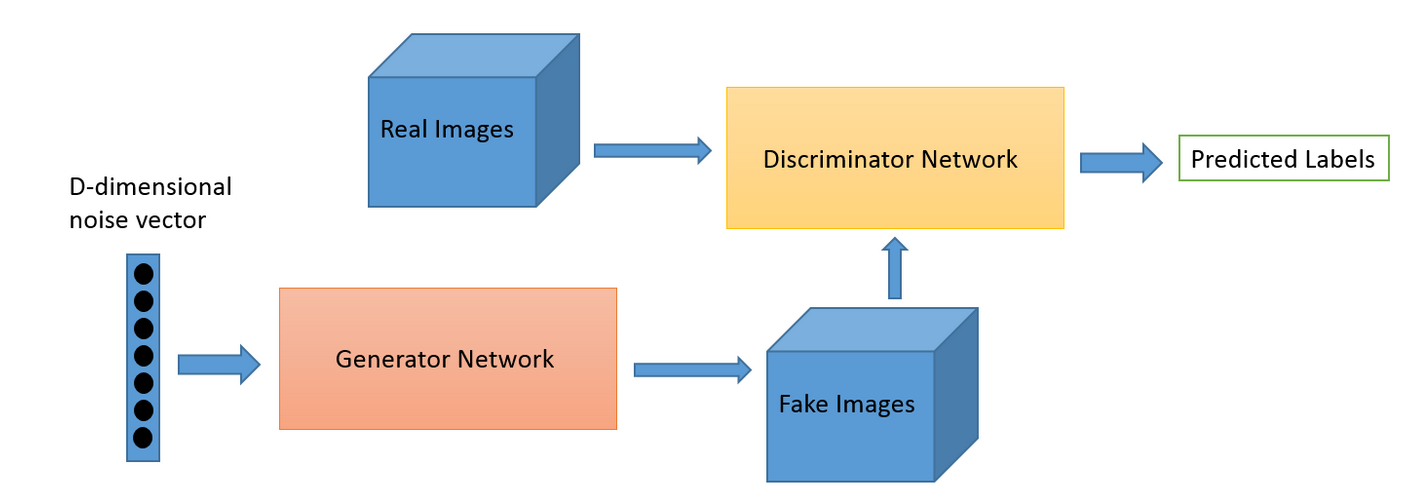
\includegraphics[scale=0.3]{./tex/generative-adversarial-network/ganpic.png}
    \caption{Architecture d'un réseau antagoniste génératif}
    \label{ganarchi}
\end{figure}

\paragraph{Fonction de perte}

\noindent Supposons:
\begin{itemize}
    \item $p_y$, distribution du \textit{bruiteur} associée à une entrée y
    \item $p_r$, distribution associée aux données réelles $x_{real}$
    \item D, fonction représentant le Discriminateur
    \item G, fonction représentant le Générateur
\end{itemize}

\noindent Dans un premier temps, nous voulons que le Discriminateur donne une forte probabilité d'être valide à une donnée réelle. Nous voulons donc que $D(x_{real}) \rightarrow 1$. Ainsi, nous pouvons considérer la fonction:
$$E_{x \sim p_r(x_{real})}[log(D(x)]$$
$$E_{x \sim p_r(x_{real})}[log(D(x)] \rightarrow 0 \  si \  D(x_{real}) \rightarrow 1$$

\noindent De même, nous voulons que le Discriminateur prédise une faible probabilité d'être valide pour une donnée artificielle soit $D(G(y)) \rightarrow 0$. Nous obtenons alors la fonction:
$$E_{y \sim p_y(y)}[log(1-D(G(y))]$$

\noindent Nous obtenons notre fonction de perte définie par:
$$L(D,G)={E}_{x \sim p_{r}(x_{real})} [\log D(x)] + {E}_{y \sim p_y(y)} [\log(1 - D(G(y)))]$$

\noindent Une particularité importante est à remarquer. La fonction L est comparable au \textbf{négatif} de la fonction \textit{Cross-Entropy}. Ainsi, pour l'apprentissage du Discriminateur, il est nécessaire de réaliser une optimisation par \textit{gradient ascent} et non une descente de gradient standard car la "minimisation" de l'erreur du Discriminateur revient à maximiser cette fonction et non la minimiser comme pratiqué classiquement en Deep Learning. En effet, $L(D,G) \leq 0$.\\

\noindent Au contraire, pour l'apprentissage du Générateur, nous souhaitons une valeur élevée pour D(G(y)). Nous pouvons réutiliser la fonction $E_{y \sim p_y(y)}[log(1-D(G(y))]$. L'apprentissage de ce réseau s'oppose ainsi à celui du Discriminateur et se basera sur la minimisation de la fonction de perte.\\

\noindent Le Générateur et le Discriminateur cherchent à optimiser deux fonctions de pertes \textbf{opposées}. Nous pouvons ainsi définir un jeu \textit{minimax} basé sur la probabilité que la donnée artificielle soit considérée comme vrai.\\

\noindent En unifiant les différentes conditions, nous obtenons:
$$\begin{aligned}
\min_G \max_D L(D, G)
& = {E}_{x \sim p_{r}(x_{real})} [\log D(x)] + {E}_{y \sim p_y(y)} [\log(1 - D(G(y)))] \\
\end{aligned}$$
\noindent Plus spécifiquement, l'apprentissage se fait en alternant l'optimisation des sous-réseaux indépendamment l'un de l'autre selon les fonctions suivantes:
\begin{itemize}
    \item Generateur: descente de gradient
    $$\min_G {E}_{y \sim p_y(y)} [\log(1 - D(G(y)))]$$
    \item Discriminateur: gradient ascent
    $$\max_D {E}_{x \sim p_{r}(x_{real})} [\log D(x)] + {E}_{y \sim p_y(y)} [\log(1 - D(G(y)))] $$
\end{itemize}

\noindent L'alternance de l'apprentissage peut être de 1(D):1(G) ou de k:1. De nombreux chercheurs ont observé expérimentalement que l'apprentissage était plus stable avec un apprentissage plus soutenu du Discriminateur. La stabilité des GAN est une des problématiques majeures de ce type d'architecture car il est difficile de faire apprendre mutuellement deux réseaux. Si l'un des deux modèles dominent l'autre, la performance de l'ensemble deviendra mauvaise. La création de fonctions de perte plus performantes est un sujet de recherche toujours très actif.\\

\noindent Dans les faits, la fonction de perte du Générateur est problématique. En effet, cette fonction ne permet pas à G d'apprendre efficacement. Lorsque le Générateur produit un faux et que ce dernier est détecté, il est nécessaire que le Générateur apprenne efficacement de son erreur. Or, la valeur du gradient tend à être infinitésimal lorsque la fonction de perte tend vers 0, cas obtenu lorsque la probabilité D(G(z)) est nulle. Au contraire, le gradient augmente lorsque le Générateur produit des faux capables de tromper le Discriminateur. Ce comportement est inadéquat car il ne permet pas au Générateur de bien apprendre lorsqu'il n'a aucune connaissance. Sur la courbe bleue de la Figure \ref{gangrad}, nous pouvons observer le comportement du gradient selon la probabilité prédite par le Discriminateur.\\

\noindent Une alternative consiste à exploiter $\log(D(G(z)))$. L'approche du comportement du Discriminateur vis-à-vis du Générateur est inversée. Au lieu de minimiser la probabilité que le Discriminateur détecte le faux, on cherchera à maximiser le fait que le Discriminateur se trompe sur sa prédiction. Nous obtenons:
$$\begin{aligned}
\max_G {E}_{y \sim p_y(y)} [\log(D(G(y)))]
\end{aligned}$$

\noindent Le comportement du gradient de la nouvelle fonction de perte du Générateur est visible sur la courbe verte de la Figure \ref{gangrad}. On peut observer que le comportement du gradient est inversé et qu'il favorise l'apprentissage lorsque le modèle est peu performant.

\noindent

\begin{figure}
    \centering
    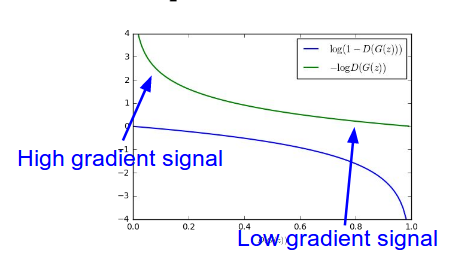
\includegraphics[scale=0.4]{./tex/generative-adversarial-network/gangrad.png}
    \caption{Comparaison des gradients de la fonction de perte du Générateur}
    \label{gangrad}
\end{figure}


\subsection{Difficultés d'apprentissage}
Bien que très puissants, les réseaux GAN sont reconnus comme étant difficiles à entraîner. En effet:\\

\begin{itemize}
    \item \textbf{Convergence}: Le risque de non-convergence est important avec ce type de réseau. L'apprentissage est alors caractérisé par un comportement très oscillant qui a tendance à finir par diverger.\\

    \item \textbf{Diversité}: Les images générées par les GAN ont tendance à être très similaires et à manquer de diversité malgré un jeu de données d'apprentissage représentatif.\\

    \item \textbf{Génération aléatoire}: Il n'est pas possible de maîtriser la génération d'images. Le comportement est exclusivement aléatoire (contrairement aux \textit{ Variationnal Autoencoderr}).\\

    \item \textbf{Equilibre des réseaux}: Pour que le réseau GAN fonctionne, il est nécessaire que le Générateur et le Discriminateur soit globalement aussi performant l'un que l'autre. Si l'un des modèles domine l'autre, le GAN ne sera pas capable de fonctionner (et d'apprendre) convenablement.\\

    \item \textbf{Hypersensibilité}: Les architectures GAN sont très dépendantes d'hyperparamètres difficiles à évaluer et sont sujets au sur-apprentissage\\
\end{itemize}

\noindent Ces differentes contraintes ont été la source d'une recherche active, notamment au niveau de la fonction de perte qui, dans sa version initiale, est globalement peu performante. De nombreuses améliorations ont été proposées à ce niveau notamment le \textit{Wasserstein GAN}\cite{wasserstein} qui repose sur la \textit{distance Wasserstein}\footnote{Cette métrique permet d'évaluer la distance entre deux distributions de probabilités.}.

\subsection{Deep Convolutional Generative Adversarial Networks (DCGAN)}
Les réseaux DCGAN\cite{dcgan}, contrairement aux réseaux GAN classiques, exploitent une architecture convolutive profonde pour le Générateur et le Discriminateur. Le Discriminateur repose sur les structures convolutives classiques telles que Inception, ResNet ou encore VGG. Une particularité notable est le remplacement des couches de Pooling par des convolutions avec un stride supérieur à 1 qui permettent d'avoir une réduction de dimension moins agressive en terme de perte d'informations. Au contraire, le Générateur repose sur des méthodes de \textit{Upsampling} afin de pouvoir générer une image qui est de dimension supérieure au signal bruité exploité comme source génératrice. La méthode standard de \textit{Upsampling} est la \textit{Convolution transposée} (aussi appelée Déconvolution\footnote{Appellation abusive}).
